%%\setchapterimage{Fond_SLCI.png}
%\setchapterpreamble[u]{\margintoc}
%\chapter{Algorithmes dichotomiques}
%
%%\marginnote[5cm]{
%%\UPSTIcompetence[2]{C1-02}
%%\UPSTIcompetence[2]{C2-04}
%%}
%
%%\marginnote[4cm]{\textbf{Qui}, \textit{Quoi}, Où.}

\newpage
\section{Algorithmes dichotomiques}
\subsection{Introduction}
Les méthodes de résolutions par un algorithme dichotomique font partie des algorithmes basés sur le principe de << diviser pour régner >>.
Elles utilisent la définition du terme \textbf{dichotomie} qui signifie diviser un tout en deux parties << opposées >>.
Certains algorithmes de tris sont basés sur ce principe de diviser pour régner.



Ce cours vous présente deux algorithmes dichotomiques :
\begin{itemize}
\item la recherche d'un élément dans une liste triée ;
\item la détermination de la racine d'une fonction quand elle existe.
\end{itemize}

\subsection{Recherche dichotomique dans une liste {triée}}

Lorsque vous cherchez le mot <<~hippocampe~>> dans le dictionnaire, vous ne vous amusez pas à parcourir chaque page depuis la lettre a jusqu'à tomber sur le mot <<~hippocampe~>>...\\
Dans une liste triée, il y a plus efficace ! Par exemple dans le dictionnaire, vous ouvrez à peu près au milieu, et suivant si le mot trouvé est \og inférieur \fg \ ou \og supérieur \fg \ à <<~hippocampe~>> (pour l'ordre alphabétique), vous poursuivez votre recherche dans l'une ou l'autre moitié du dictionnaire.


\begin{prop}
On se donne une liste \lstinline{L} de nombres de longueur \lstinline{n},     {triée dans l'ordre croissant}, et un nombre \lstinline{x0}. 

Pour chercher \lstinline{x0}, on va couper la liste en deux moitiés et chercher dans la moitié intéressante et ainsi de suite.

On appelle \lstinline{g} {l'indice} de l'élément du début de la sous-liste dans laquelle on travaille et \lstinline{d}     {l'indice} de l'élément de fin.

Au début, \lstinline{g = 0} et \lstinline{d = n-1} 

On souhaite construire un algorithme admettant l'invariant suivant:
\bigskip

\centerline{{si \lstinline{x0} est dans \lstinline{L} alors \lstinline{x0} est dans la sous-liste \lstinline{L[g:d]} (\lstinline{g} inclus et \lstinline{d} exclu).}}
\end{prop}



On va utiliser la méthode suivante.
\begin{itemize}
\item On compare \lstinline{x0} à <<~l'élément du milieu~>> : c'est \lstinline{L[m]} où \lstinline{m = (g+d)//2}
son indice est \lstinline{m} =\lstinline{ n//2} (division euclidienne)
%$$\begin{array}{|c|c|c|c|c|c|c|c|c|} 
%\hline \hspace*{3mm} & \hspace*{3mm} & \hspace*{3mm} &  \hspace*{3mm} & \hspace*{3mm} & \hspace*{3mm} & \hspace*{3mm} & \hspace*{3mm} & \hspace*{3mm}\\ \hline
%\end{array}$$
%\medskip
%$$\begin{array}{|c|c|c|c|} 
%\hline \hspace*{3mm} & \hspace*{3mm} & \hspace*{3mm} &  \hspace*{3mm} \\ \hline
%\end{array}$$

\item Si \lstinline{x0 = L[m]}, on a trouvé \lstinline{x0}, on peut alors s'arrêter.
\item Si \lstinline{x0} $<$ \lstinline{L[m]}, c'est qu'il faut chercher dans la première moitié de la liste, entre \lstinline{L[g]} et  \lstinline{L[m-1]} (\lstinline{L[m]} exclu).
%dans  {la première moitié de la liste \t{L[g:m]}}\\
\item Si \lstinline{x0} $>$ \lstinline{L[m]}, c'est qu'il faut chercher dans la seconde moitié de la liste, entre \lstinline{L[m+1]} et \lstinline{L[d]} (\lstinline{L[m]} exclu).
\end{itemize}

On poursuit jusqu'à ce qu'on a trouvé \lstinline{x0} ou lorsque l'on a épuisé la liste \lstinline{L}.



\newpage


\subsubsection{Exemples d'application}
%\begin{enumerate}
%\item %En notant $g$ et $d$  les indices de gauche et de droite du morceau de la liste $l$ où l'on est en train de faire la %recherche, 


Indiquer pour les deux exemples suivants les valeurs successives de \lstinline{g} et \lstinline{d} :
\begin{enumerate}
\item \lstinline{x0 = 5} et \lstinline{L} $= \begin{array}{|c|c|c|c|c|c|c|c|c|} 
\hline -3 & 5 & 7 & 10 & 11 & 14 & 17 & 21 & 30 \\ \hline
\end{array}$

\marginnote{Cas 1 :
$\begin{cases}
g=0\\d=8\\m=4,L[m]>x0
\end{cases}$
$\begin{cases}
g=0\\d=3\\m=1,L[m]=x0
\end{cases}$.\\
C'est fini, on a bien trouvé $x_0$ dans la liste.}

\marginnote{Cas 2 :
$\begin{cases}
g=0\\d=8\\m=4,L[m]<x0
\end{cases}$, $\begin{cases}
g=5\\d=8\\m=6,L[m]>x0
\end{cases}$ $\begin{cases}
g=5\\d=5\\m=5,L[m]<x0
\end{cases}$ $\begin{cases}
g=6\\d=5
\end{cases}$.
C'est fini, on a épuisé la liste \lstinline{L} et on n'a pas trouvé $x0$.}


\item \lstinline{x0 = 11} et \lstinline{L} $= \begin{array}{|c|c|c|c|c|c|c|c|c|} 
\hline -2 & 1 & 2 & 7 & 8 & 10 & 13 & 16 & 17  \\ \hline
\end{array}$

\end{enumerate}


%\textbf{Remarque :} On en déduit que de manière générale, \lstinline{m = (g + d) // 2} (division euclidienne)\\
 %- si \lstinline{x0} $<$ \lstinline{L[m]}, \lstinline{g} est inchangé et \lstinline{d} prend la valeur de \lstinline{m}\\
 %- si \lstinline{L[m]} $\leq$ \lstinline{x0}, \lstinline{d} est inchangé et \lstinline{g} prend la valeur de \lstinline{m}
 

\subsubsection{Implémentation en Python}
La fonction \lstinline{recherche_dichotomie} d'arguments une liste \lstinline{L} et un élément \lstinline{x} renvoyant un booléen disant si \lstinline{x} est dans la liste \lstinline{L} est proposée :


\begin{lstlisting}
def recherche_dichotomie(L:list, x:int)-> bool:
    n = len(L)
    g = 0 # c'est l'indice de gauche
    d = n - 1 # c'est l'indice de droite
    rep = False
    while g <= d and rep == False :
        # si x est dans L alors L[g] <= x <= L[d]     {invariant}
        m = (g+d) // 2 
        if x == L[m]:
            rep = True
        elif x < L[m]:
            d = m - 1
        else:
            g = m + 1
        # si x est dans L alors L[g] <= x <= L[d]     {invariant}
    return(rep)
\end{lstlisting} 



%\begin{python}
%def dichotomie(L, x0):\\
%     n = len(L)\\
%     g = 0\\
%     d = n\\
%     while  {d - g > 1:}\\
%         m =  {(d + g) // 2} \\
%         if  {x0 < L[m]}\\
%              {d = m}\\
%          else:\\
%              {g = m}\\
%     return  {x0 == L[g]}
%\end{python}
\textbf{Remarque :} La terminaison de l'algorithme est obtenue avec $d-g$ qui est un entier positif qui décro\^{i}t strictement à chaque passage dans la boucle \lstinline{while} et joue le rôle de variant.
%\end{enumerate}

\subsubsection{Implémentation récursive}
\begin{lstlisting}
def recherche_dichotomique_recursive(L:[int], x0:int, g:int, d:int) -> bool:
    if g>d : 
        return False # ou -1
    m = (g+d)//2
    if L[m] == x0 :
        return True # ou m
    elif L[m] > x0 :
        return recherche_dichotomique_recursive(L, x0, g, d-1)
    else :
        return recherche_dichotomique_recursive(L, x0, g+1, d)
\end{lstlisting} 


\subsubsection{Terminaison (Implémentation non récursive)}

Prenons comme variant de boucle la longeur de la zone de recherche, à savoir, à la n\ieme itération, 
$\ell_n = d_n - g_n$. 

À l'itération suivante, $ m_{n+1} =  \left\lfloor \dfrac{g_n+d_n}{2}  \right\rfloor$
\begin{itemize}
\item ou bien \lstinline{L[m]==x0} et l'alogrithme s'arrête;
\item ou bien  $g_{n+1} = g_n$ et $d_{n+1} = m_{n+1}-1$. Ainsi, $\ell_{n+1} =  \left\lfloor \dfrac{g_n+d_n}{2}  \right\rfloor-1 -  g_n$ et 
$\ell_{n+1} \leq   \dfrac{g_n+d_n}{2}  -1 -  g_n $ $ \leq   \dfrac{g_n+d_n - 2 - 2g_n }{2}  $ $ \leq   \dfrac{\ell_n- 2 }{2}  $  $< \ell_n$;
\item ou bien  $g_{n+1} =  m_{n+1}+1$ et $d_{n+1} = d_n$.
 Ainsi, $\ell_{n+1} =  d_n  - \left\lfloor \dfrac{g_n+d_n}{2}  \right\rfloor-1$ et 
$\ell_{n+1} \leq   d_n  -  \dfrac{g_n+d_n}{2}  -1 $  
$\leq   \dfrac{2 d_n - g_n - d_n}{2}  -1 $  
$< \ell_n $.
\end{itemize}

La longueur $\ell_n$ est donc strictement décroissante. L'algorithme terminera donc. 

\subsubsection{Preuve de correction (Implémentation non récursive)}

Montrons que \lstinline{x} $\in$ \lstinline{L} $\Rightarrow$ \lstinline{x} $\in$ \lstinline{[g:d+1]}.\sidenote{Cela signifie que $x\in\llbracket g,d\rrbracket$.}

\begin{itemize}
\item En entrant dans la boucle, $g=0$ et $d+1=n-1+1=n$. Si \lstinline{x} $\in$ \lstinline{L} alors, \lstinline{x} $\in$ \lstinline{[0:n]}. La propriété d'invariance est donc vérifiée.

\item Considérons la propriété 
\lstinline{x} $\in$ \lstinline{L} $\Rightarrow$ \lstinline{x} $\in$ \lstinline{[g:d+1]}
est vraie à la \ieme itération.

\item On calcule \lstinline{m}.

\item Si \lstinline{x = L[m]}, on a bien \lstinline{x} $\in$ \lstinline{[g:d+1]}. La propriété d'invariance est vérifiée à la fin de l'itération et on sort de la boucle (car \lstinline{rep} est \lstinline{True}). 

\item Si \lstinline{x < L[m]}, on a déjà vérifié que \lstinline{x} était différent de \lstinline{L[m]} et alors \lstinline{d=m-1}. Donc $g=g$ et $d+1=m-1+1=m$.
\lstinline{x} $\in$ \lstinline{L} alors \lstinline{x} $\in$ \lstinline{[g:m]}. La propriété d'invariance est donc vérifiée.

\item Si \lstinline{x > L[m]}, on a déjà vérifié que \lstinline{x} était différent de \lstinline{L[m]} et alors \lstinline{g=m+1}. Donc $g=m+1$ et $d+1$ est inchangé.
 Donc si 
\lstinline{x} $\in$ \lstinline{L} alors \lstinline{x} $\in$ \lstinline{[m+1:d+1]}. La propriété d'invariance est donc vérifiée.
\end{itemize}
Dans chacun des cas, la propriété d'invariance est vérifiée à la fin de la \ieme itération. C'est donc bien un invariant de boucle. 

\subsection{Analyse de la complexité}
Dans le pire des cas, le terme recherché n'est pas dans la liste. On divise donc la taille du tableau par 2 tant que la taille est supérieure ou égale à 1. 

On note $n$ la taille du tableau. On cherche $k$ le nombre de fois qu'on peut diviser la taille du tableau par 2 : 
$n\cdot\left(\dfrac{1}{2}\right)^k \geq 1$ 
$\Rightarrow \cdot\left(\dfrac{1}{2}\right)^k \geq \dfrac{1}{n}$
$\Rightarrow k \ln\left(\dfrac{1}{2}\right) \geq \ln\left(\dfrac{1}{n}\right)$
$\Rightarrow k \geq \dfrac{\ln\left(\dfrac{1}{n}\right)}{\ln\left(\dfrac{1}{2}\right)}$
$\Rightarrow k \geq \dfrac{\ln n}{\ln 2}$.
Il y aura donc dans le pire des cas $\log_2 n$ opérations.  L'algorithme de recherche dichotomique est donc en $\mathcal{O}(\log_2(n))$.

\subsection{Détermination de la racine d'une fonction par dichotomie}

\subsubsection{Principe théorique de la méthode par dichotomie}
%
\begin{marginfigure}
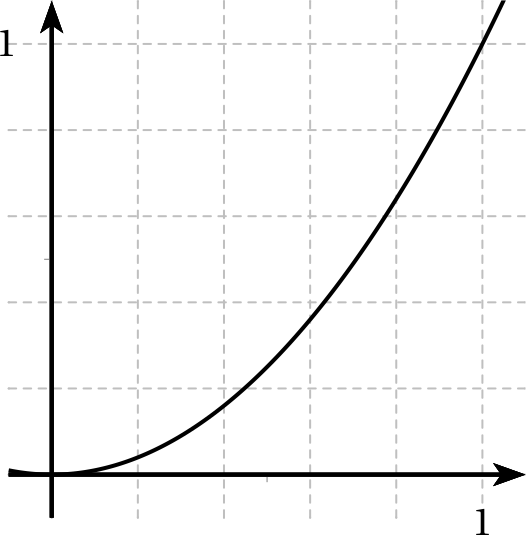
\includegraphics[width=\linewidth]{courbe}
\end{marginfigure}
% 
On considère une fonction $f$ vérifiant : 
\begin{center} $f$ continue sur $\verb![!a,b\verb!]!$ ;  $f(a)$ et $f(b)$ de signes opposés.
\end{center} Le théorème des valeurs intermédiaires nous assure que $f$ possède au moins un zéro $\ell$ entre $a$ et $b$. La preuve, vue en cours de mathématiques, repose sur la méthode de dichotomie. Prenons le cas $f(a)<0$ et $f(b)>0$ et posons $g_0=a$, $d_0=b$. 


 On considère $m_0 = \dfrac{g_0+d_0}{2}$ et on évalue $f(m_0)$ : 
\begin{itemize}
 \item Si $f(m_0)\geq 0$, on va poursuivre la recherche d'un zéro dans l'intervalle  {$[g_0,m_0]$} \\On pose donc  : 
 $g_1 =  {g_0} \quad ;\quad  d_1 =  {m_0}$\vspace*{2mm}
  \item Sinon,  la recherche doit se poursuivre  dans l'intervalle  {$[m_0,d_0]$} \\ On pose donc  : 
 $g_1 =  {m_0} \quad ; \quad d_1 =  {d_0}$\vspace*{2mm}
 \item On recommence alors en considérant $m_1 = \dfrac{g_1+d_1}{2}$...\\
 \end{itemize}

%
% \begin{enumerate}
% \item Par quoi peut-on remplacer la condition "$f(m_k)\geq 0$" dans le cas général où $f(a)$ et $f(b)$ sont de signes contraires (pas forcément $f(a)<0$ et $f(b)>0$) ?
%
% \item \`A quelle condition sur $g_n$ et $d_n$ s'arrête-t-on, si l'on souhaite que $g_n$ et $d_n$ soient des solutions approchées de $\ell$ à une précision $\varepsilon$ ?
%
% \item  Au lieu de renvoyer $g_n$ et/ou $d_n$ comme valeurs approchées de $\ell$, que pourrait-on prendre ? 
% 
% Que mettre comme condition d'arrêt pour avoir une précision $\varepsilon$  ? 
%
% \item Un étudiant propose de tester si $f(m_k)=0$.  Qu'en pensez-vous ?
%
%\end{enumerate}


\subsubsection{Implémentation en Python et avec scipy}
\'Ecrivons une fonction \lstinline{zero_dichotomie(f:callable, a:float, b:float, epsilon:float) -> float} d'arguments une fonction \lstinline{f}, des flottants \lstinline{a} et \lstinline{b} (tels que \lstinline{a < b}), et  la précision voulue \lstinline{epsilon} (flottant strictement positif). Cette fonction renverra une valeur approchée à \lstinline{epsilon} près d'un zéro de \lstinline{f}, compris entre \lstinline{a} et \lstinline{b}, obtenue par la méthode de dichotomie.

\begin{lstlisting}
def zero_dichotomie(f:callable, a:float, b:float, epsilon:float) -> float:
    g = a # c'est un flottant
    d = b # c'est un flottant
    while d-g > 2*epsilon :
        m = (g + d) / 2
        if f(g)*f(m) <= 0:
            d = m
        else:
            g = m
    return ((g + d)/2)
\end{lstlisting}

Effectuons un test avec la fonction $f : x \mapsto x^2-2$ sur l'intervalle $\verb![!1,2\verb!]!$, avec une précision de $10^{-6}$ :
 
\begin{lstlisting}
def f(x):
     return(x ** 2 - 2)
print (zero dichotomie(f, 1, 2, 10**(-6)))

# il s'affichera : 1.4142141342163086
\end{lstlisting}
%\begin{algorithm}
%\begin{algorithmic}
%
% {
%\STATE $g \leftarrow a$
%\STATE $d \leftarrow b$
%\WHILE{$d-g> 2\varepsilon$}
%\STATE $m \leftarrow (g+d)/2$
%\IF{$f(g)f(m)\leq 0$}
%\STATE $d \leftarrow m$
%\ELSE
%\STATE $g \leftarrow m$
%\ENDIF
%\ENDWHILE
%\STATE renvoyer $\dfrac{g+d}{2}$}
%~\newline
%~\newline
%~\newline
%\end{algorithmic}
%\end{algorithm}
% 

%\subsection{Fonction prédéfinie dans scipy}
Une telle fonction est déjà prédéfinie dans la bibliothèque \lstinline{scipy.optimize}, la fonction \lstinline{bisect}\sidenote{La méthode de dichotomie s'appelle aussi la méthode de la \textit{bisection}.} : 
\begin{lstlisting}
import scipy.optimize as spo
print (spo.bisect(f, 1, 2)) 
# il s'affichera : 1.4142135623724243
\end{lstlisting}
La précision est un argument optionnel (à mettre après \lstinline{f}, \lstinline{a} et \lstinline{b}) et vaut $10^{-12}$ par défaut.

